\section{Experimental Results}
\label{sec:exp}
\begin{figure*}[t]
	\centering
	\begin{subfigure}{0.4\columnwidth}
		\centering
		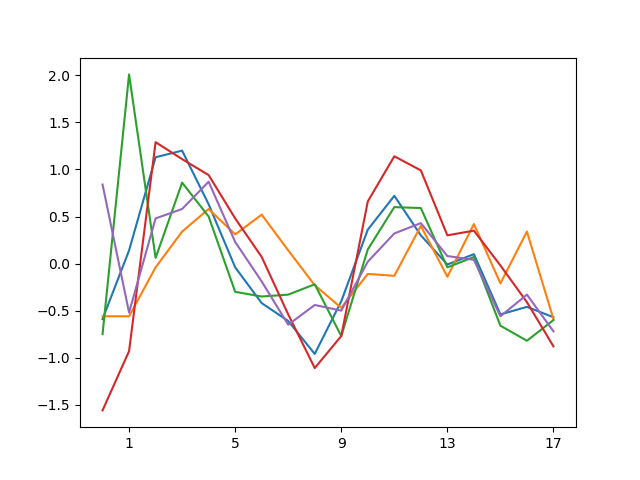
\includegraphics[width=\columnwidth, height=4 cm]{Figures/yeast_G1.png}
		\caption{yeast G1 phase}
	\end{subfigure}%
	\begin{subfigure}{0.4\columnwidth}
		\centering
		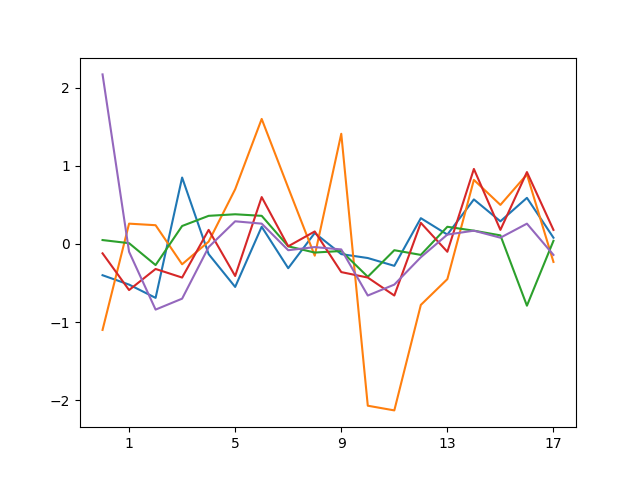
\includegraphics[width=\columnwidth, height=4 cm]{Figures/yeast_G2.png}
		\caption{yeast G2 phase}
	\end{subfigure}%
	\begin{subfigure}{0.4\columnwidth}
		\centering
		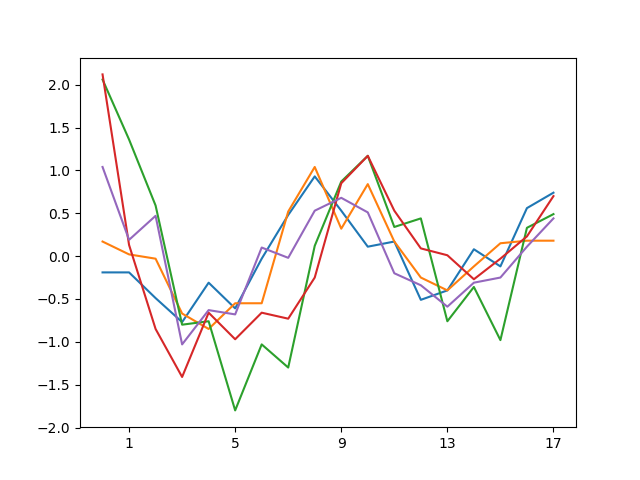
\includegraphics[width=\columnwidth, height=4 cm]{Figures/yeast_M.png}
		\caption{yeast M phase}
	\end{subfigure}
		\begin{subfigure}{0.4\columnwidth}
		\centering
		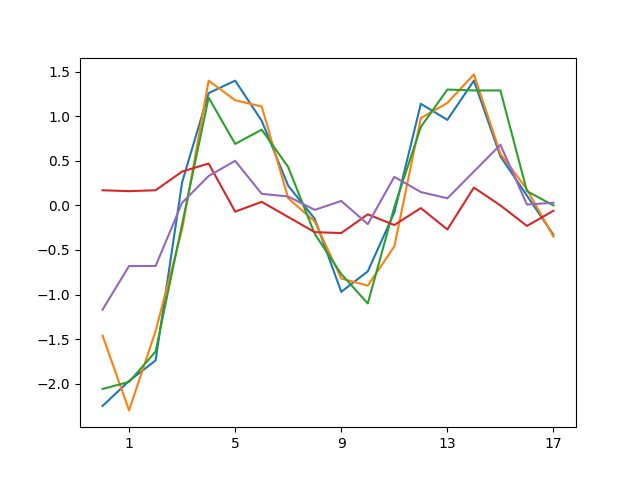
\includegraphics[width=\columnwidth, height=4 cm]{Figures/yeast_S.png}
		\caption{yeast S phase}
	\end{subfigure}
		\begin{subfigure}{0.4\columnwidth}
		\centering
		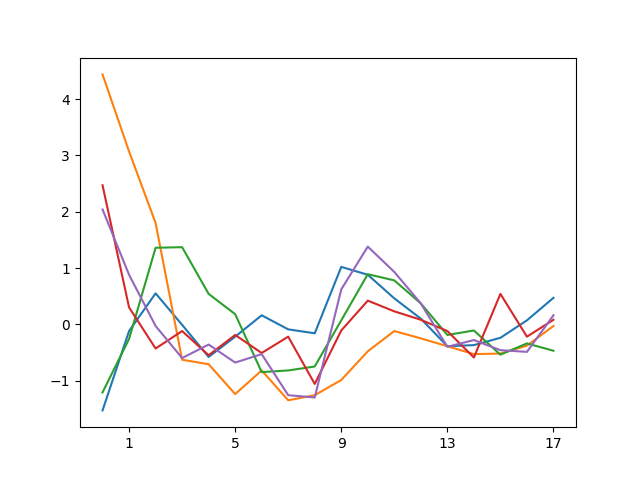
\includegraphics[width=\columnwidth, height=4 cm]{Figures/yeast_M_G1.png}
		\caption{yeast M/G1 phase}
	\end{subfigure}
	\caption{Different phase of yeast gene expression}
	\label{fig-yeast_data}
\end{figure*}

We run various experiments on different methods of anomaly detection and  forecasting over two real datasets. Distinct performance metrics are used in different methods. 
In this section we briefly describe the datasets used and experimental setup for performance analysis on the approaches as discussed in previous sections.

\subsection{Datasets}
We use two real datasets in our experiments and each dataset contains different number of genes and their associated time values of equal or unequal length.

\paragraph*{\textbf{Yeast}} The first dataset considered in our tests, denoted as \textbf{Yeast} and originally described in \cite{first_dataset}, contains the genome characterization of the mRNA transcript levels during the cell cycle of the yeast \textit{Saccharomyces cerevisiae}. Gene expression levels were gathered at regular intervals during the cell cycle. In particular, measurements were performed at $17$ time points with an interval of $10$ minutes between each pair of recorded values. Different experiments are done in the gene expression time series of this dataset are known to be associated to $5$ different phases, namely \texttt{Early G1/M}, \texttt{G1}, \texttt{S}, \texttt{G2} and \texttt{M} which represent the class values in their setting. From the dataset, there are 87 genes that are labelled with these distinct phases. Therefore, we only consider these gene expression in our problem.  Figure \ref{fig-yeast_data} shows sample gene expression for various phases in this dataset.


\paragraph*{$\mathbf{MS-rIFN\beta}$}
The second dataset, indicated as $\mathbf{MS-rIFN\beta}$ or $\mathbf{patient}$ data in short and first analyzed in \cite{second_dataset}. It contains gene expression profiles of 52 patients suffering from relapsing-remitting multiple sclerosis (MS), who are classified as either good (33) or poor (19) responders to recombinant human interferon beta (rIFN$\beta$). The dataset is composed by the expression profiles of $70$ genes isolated from each patient at $7$ time points: before the administration of the first dose of the drug ($t= 0$), every $3$ months ($t=1, 2, 3, 4$) and every $6$ months ($t=5,6$) in the first and second year of the therapy, respectively. For a few patients entire profile measurements are missing at $1$ or $2$ time points. We consider gene  from each parent as separate identity and therefore we get 3640 gene expressions in total. We make each expression in equal length of nine by fitting the missing values with interpolation. We normalise the expression to prepare thme for the model.

\begin{figure}[]
	\centering
	\begin{subfigure}{0.5\columnwidth}
		\centering
		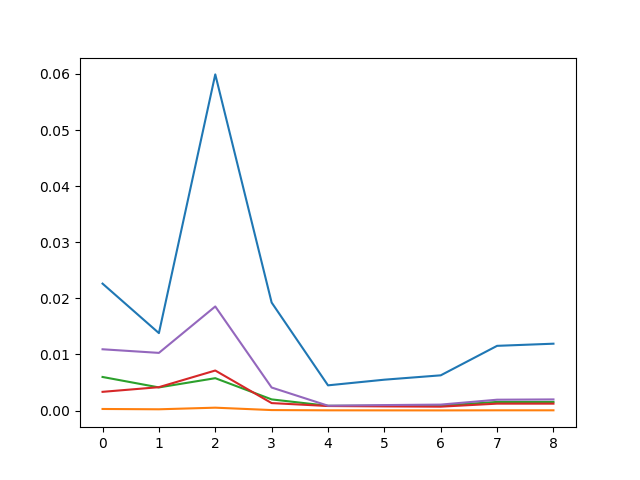
\includegraphics[width=\columnwidth, height=4 cm]{Figures/patient_good_gene.png}
		\caption{Good gene expression}
	\end{subfigure}%
	\begin{subfigure}{0.5\columnwidth}
		\centering
			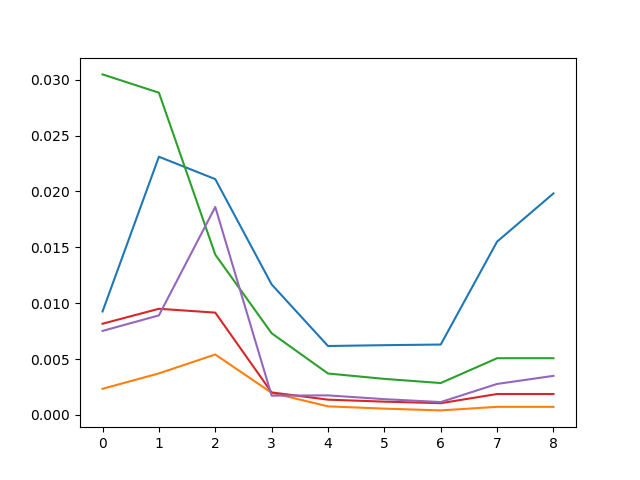
\includegraphics[width=\columnwidth, height=4 cm]{Figures/patient_bad_gene.png}
		\caption{Bad gene expression}
	\end{subfigure}%
	\caption{Sample Gene expression from patient dataset}
	\label{fig-patient_data}
\end{figure}

\subsection{Environment Setup}
All of our experiments are implemented in Python. Moreover, we use external packages and library for various methods.  Supervised and unsupervised machine learning based models for anomaly detection have been implemented with Python machine learning packages scikit-learn\footnote{\url{http://scikit-learn.org/stable/}}.

We use Statsmodels\footnote{\url{http://www.statsmodels.org/stable/index.html}} for ARIMA model in forecasting. For deep-learning based LSTM and Neural Network method, we use Python Deep Learning library Keras\footnote{\url{https://keras.io/}} using Tensorflow\footnote{\url{https://www.tensorflow.org/}} as backend.

Experimental evaluation was conducted on a
machine with a Intel core i7 processor with 2.5GHz clock speed and 16GB RAM. The machine has also a Nvidia GTX 960M with 4GB memory and therefore
Tensorflow based experiments can utilize GPU instructions.


\subsection{Anomaly detection performance}

All the methods in anomaly detection finds out the anomalous gene expression from the normal ones. In \textit{patient} dataset, we consider the gene expression labelled with 'bad' responder as anomalous and  'good' responder as normal expression. On the other hand, in \textbf{yeast} dataset gene expression are classified into different phases. Therefore, we run one vs all methods to detect anomaly in gene expression. Each time we consider each phase as anomalous expression and the rest are normal. 

For each experiment, we keep 80\% data for training purpose and the rest are evaluated in testing. Since each of the methods divide the input space
in normal and outlier (anomalous) portion, we use 2 class accuracy and
corresponding F1 score (from confusion matrix) as performance metric for
them. 
\begin{figure}[]
	\centering
	\begin{subfigure}{0.5\columnwidth}
		\centering
		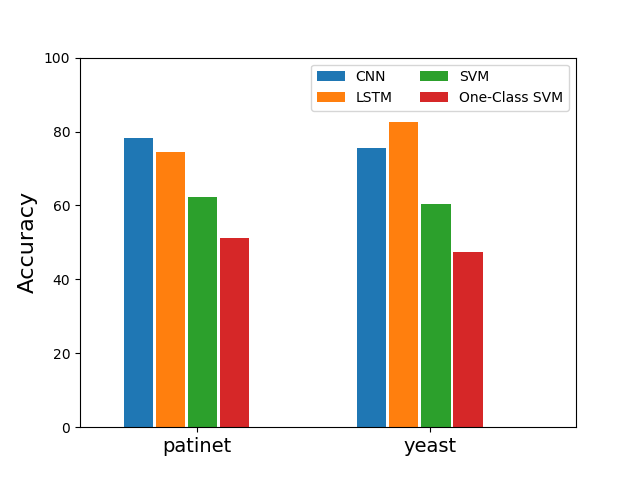
\includegraphics[width=\columnwidth, height=4 cm]{Figures/anomaly_acc.png}
		\caption{Accuracy score}
	\end{subfigure}%
	\begin{subfigure}{0.5\columnwidth}
		\centering
			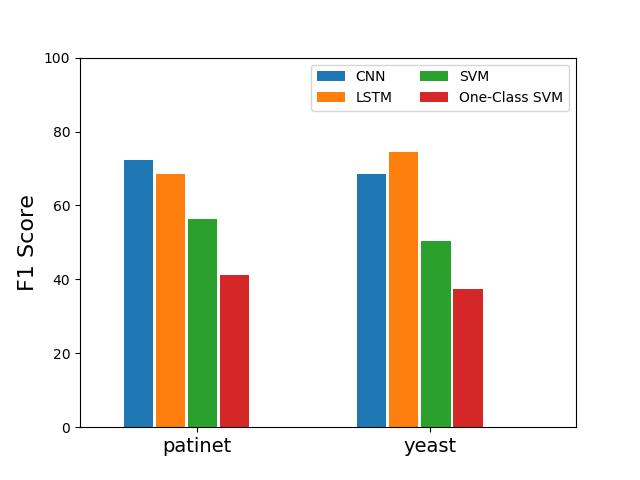
\includegraphics[width=\columnwidth, height=4 cm]{Figures/anomaly_f1.png}
		\caption{F1 score}
	\end{subfigure}%
	\caption{Anomaly detection performance of various methods}
	\label{fig-anomaly}
\end{figure}

Figure \ref{fig-anomaly} shows the performance of various anomaly detection method in our datasets. The accuracy of CNN is highest in \textit{Patient} dataset and for \textit{Yeast} dataset it is LSTM. Both of them are far better them SVM and One-class SVM. The performance of one class SVM is least in both datasets and less than 50\%. We also see the similiar performance measure in term of F1 score. 

\subsection{Forecasting Performance} 
We have used four methods, Holtz-Winter, ARIMA, Deep neural network and LSTM for forecasting. In this purpose, we divide the dataset into train and test. We build the model based on training data and compute forecasting on the rest of the portion to compare with the actual test data. We use 10\%, 20\%, 30\% and 40\% of a time series as testing data. 

For performance metric, we have used Root Mean Squared Error (RMSE). Let $x_1, x_2, \dots ,x_k$ are actual values of a time series $X$ and $k$ periods forecasting values are measured as $x'_1, x'_2, \dots ,x'_k$, then RMSE error is defined as,
\[ RMSE(X) = \sqrt{\sum{\frac{(x_i-x'_i)^2}{k}}}_{i=1}^{k}\]


Squaring the forecast error values forces them to be positive; it also has the effect of putting more weight on large errors.
Very large or outlier forecast errors are squared, which in turn has the effect of dragging the mean of the squared forecast errors out resulting in a larger mean squared error score. In effect, the score gives worse performance to those models that make large wrong forecasts.

\begin{figure}[]
	\centering
	\begin{subfigure}{0.5\columnwidth}
		\centering
		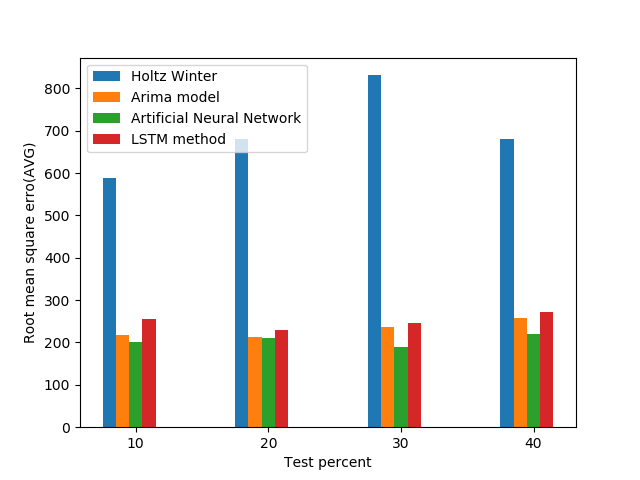
\includegraphics[width=\columnwidth, height=4 cm]{Figures/patient_forecast_rmse.png}
		\caption{Patient dataset}
	\end{subfigure}%
	\begin{subfigure}{0.5\columnwidth}
		\centering
			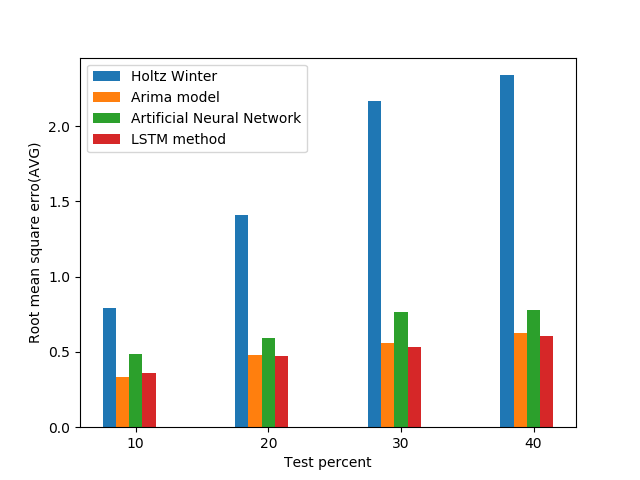
\includegraphics[width=\columnwidth, height=4 cm]{Figures/yeast_forecast_rmse.png}
		\caption{Yeast dataset}
	\end{subfigure}%
	\caption{Forecasting performance of various methods}
	\label{fig-forecast}
\end{figure}

Figure \ref{fig-forecast} shows RMSE error of different methods in all three
datasets. In all cases, Holtz winter provides maximum error.
For large scale , RMSE of of three methods other than Holtz winter do not
change significantly when test percent increase. DNN provides better result
compared to LSTM and ARIMA.
However for multi-phase yeast dataset, error of DNN is higher than
ARIMA and LSTM. Error slightly increases for all methods as test percent
increase. Performance of ARIMA and LSTM are nearly equal.